% SOURCE: edit-harness/results/frame_a/cells/cell_*_real_MIX_{A,B,C}_*.json
% !TEX encoding = UTF-8 Unicode
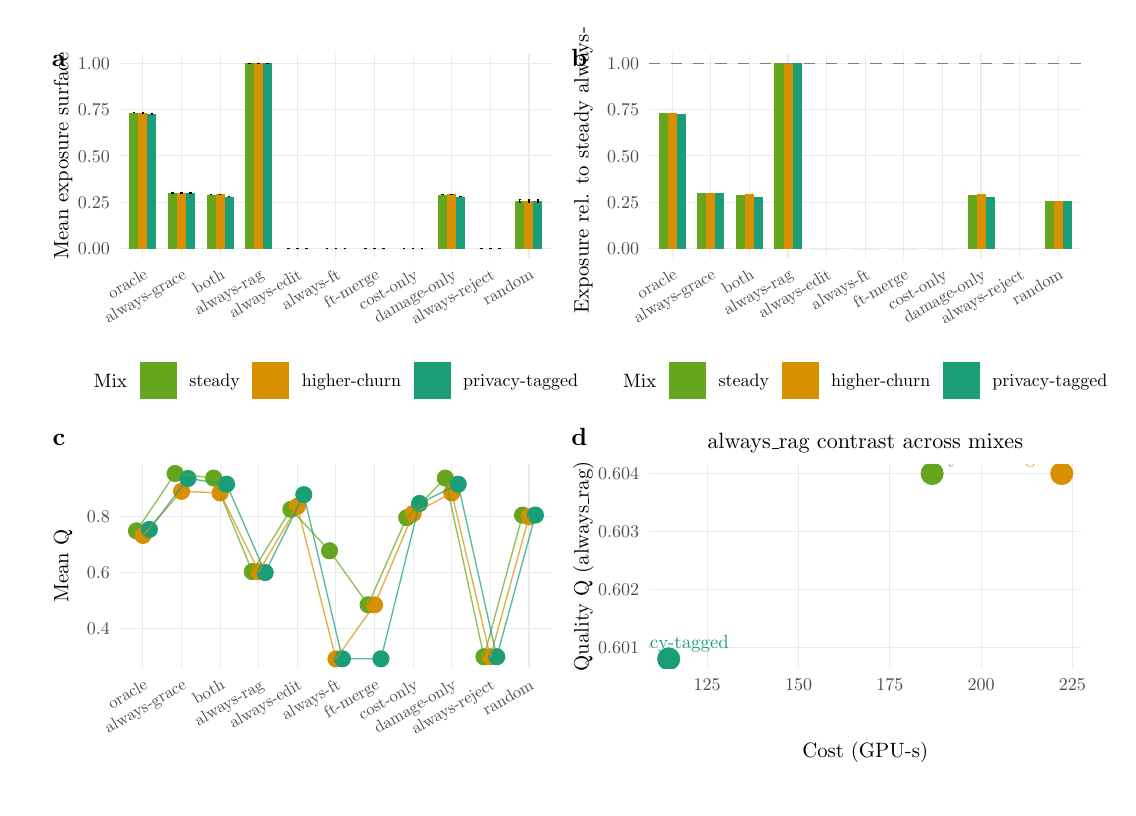
\begin{tikzpicture}[x=1pt,y=1pt]
\definecolor{fillColor}{RGB}{255,255,255}
\path[use as bounding box,fill=fillColor,fill opacity=0.00] (0,0) rectangle (390.26,274.63);
\begin{scope}
\path[clip] (  0.00,  0.00) rectangle (390.26,274.63);
\definecolor{drawColor}{RGB}{255,255,255}
\definecolor{fillColor}{RGB}{255,255,255}

\path[draw=drawColor,line width= 0.6pt,line join=round,line cap=round,fill=fillColor] (  0.00,  0.00) rectangle (390.26,274.63);
\end{scope}
\begin{scope}
\path[clip] (  5.50,131.93) rectangle (193.50,269.13);
\definecolor{fillColor}{RGB}{255,255,255}

\path[fill=fillColor] (  5.50,131.93) rectangle (193.50,269.13);
\end{scope}
\begin{scope}
\path[clip] (193.50,131.93) rectangle (384.76,269.13);
\definecolor{fillColor}{RGB}{255,255,255}

\path[fill=fillColor] (193.50,131.93) rectangle (384.76,269.13);
\end{scope}
\begin{scope}
\path[clip] (  5.50,  5.50) rectangle (193.50,131.93);
\definecolor{fillColor}{RGB}{255,255,255}

\path[fill=fillColor] (  5.50,  5.50) rectangle (193.50,131.93);
\end{scope}
\begin{scope}
\path[clip] (193.50,  5.50) rectangle (384.76,131.93);
\definecolor{fillColor}{RGB}{255,255,255}

\path[fill=fillColor] (193.50,  5.50) rectangle (384.76,131.93);
\end{scope}
\begin{scope}
\path[clip] ( 33.28,191.43) rectangle (189.50,265.13);
\definecolor{drawColor}{gray}{0.92}

\path[draw=drawColor,line width= 0.4pt,line join=round] ( 33.28,194.78) --
	(189.50,194.78);

\path[draw=drawColor,line width= 0.4pt,line join=round] ( 33.28,211.53) --
	(189.50,211.53);

\path[draw=drawColor,line width= 0.4pt,line join=round] ( 33.28,228.28) --
	(189.50,228.28);

\path[draw=drawColor,line width= 0.4pt,line join=round] ( 33.28,245.03) --
	(189.50,245.03);

\path[draw=drawColor,line width= 0.4pt,line join=round] ( 33.28,261.78) --
	(189.50,261.78);

\path[draw=drawColor,line width= 0.4pt,line join=round] ( 41.65,191.43) --
	( 41.65,265.13);

\path[draw=drawColor,line width= 0.4pt,line join=round] ( 55.59,191.43) --
	( 55.59,265.13);

\path[draw=drawColor,line width= 0.4pt,line join=round] ( 69.54,191.43) --
	( 69.54,265.13);

\path[draw=drawColor,line width= 0.4pt,line join=round] ( 83.49,191.43) --
	( 83.49,265.13);

\path[draw=drawColor,line width= 0.4pt,line join=round] ( 97.44,191.43) --
	( 97.44,265.13);

\path[draw=drawColor,line width= 0.4pt,line join=round] (111.39,191.43) --
	(111.39,265.13);

\path[draw=drawColor,line width= 0.4pt,line join=round] (125.34,191.43) --
	(125.34,265.13);

\path[draw=drawColor,line width= 0.4pt,line join=round] (139.29,191.43) --
	(139.29,265.13);

\path[draw=drawColor,line width= 0.4pt,line join=round] (153.24,191.43) --
	(153.24,265.13);

\path[draw=drawColor,line width= 0.4pt,line join=round] (167.19,191.43) --
	(167.19,265.13);

\path[draw=drawColor,line width= 0.4pt,line join=round] (181.14,191.43) --
	(181.14,265.13);
\definecolor{fillColor}{RGB}{102,166,31}

\path[fill=fillColor] ( 36.76,194.78) rectangle ( 40.02,243.92);

\path[fill=fillColor] ( 50.71,194.78) rectangle ( 53.97,214.88);

\path[fill=fillColor] ( 64.66,194.78) rectangle ( 67.92,214.31);

\path[fill=fillColor] ( 78.61,194.78) rectangle ( 81.86,261.78);

\path[fill=fillColor] ( 92.56,194.78) rectangle ( 95.81,194.78);

\path[fill=fillColor] (106.51,194.78) rectangle (109.76,194.78);

\path[fill=fillColor] (120.46,194.78) rectangle (123.71,194.78);

\path[fill=fillColor] (134.41,194.78) rectangle (137.66,194.78);

\path[fill=fillColor] (148.35,194.78) rectangle (151.61,214.31);

\path[fill=fillColor] (162.30,194.78) rectangle (165.56,194.78);

\path[fill=fillColor] (176.25,194.78) rectangle (179.51,212.04);
\definecolor{fillColor}{RGB}{216,144,0}

\path[fill=fillColor] ( 40.02,194.78) rectangle ( 43.27,243.89);

\path[fill=fillColor] ( 53.97,194.78) rectangle ( 57.22,214.88);

\path[fill=fillColor] ( 67.92,194.78) rectangle ( 71.17,214.47);

\path[fill=fillColor] ( 81.86,194.78) rectangle ( 85.12,261.78);

\path[fill=fillColor] ( 95.81,194.78) rectangle ( 99.07,194.78);

\path[fill=fillColor] (109.76,194.78) rectangle (113.02,194.78);

\path[fill=fillColor] (123.71,194.78) rectangle (126.97,194.78);

\path[fill=fillColor] (137.66,194.78) rectangle (140.92,194.78);

\path[fill=fillColor] (151.61,194.78) rectangle (154.86,214.47);

\path[fill=fillColor] (165.56,194.78) rectangle (168.81,194.78);

\path[fill=fillColor] (179.51,194.78) rectangle (182.76,212.04);
\definecolor{fillColor}{RGB}{27,158,119}

\path[fill=fillColor] ( 43.27,194.78) rectangle ( 46.53,243.52);

\path[fill=fillColor] ( 57.22,194.78) rectangle ( 60.48,214.88);

\path[fill=fillColor] ( 71.17,194.78) rectangle ( 74.43,213.51);

\path[fill=fillColor] ( 85.12,194.78) rectangle ( 88.37,261.78);

\path[fill=fillColor] ( 99.07,194.78) rectangle (102.32,194.78);

\path[fill=fillColor] (113.02,194.78) rectangle (116.27,194.78);

\path[fill=fillColor] (126.97,194.78) rectangle (130.22,194.78);

\path[fill=fillColor] (140.92,194.78) rectangle (144.17,194.78);

\path[fill=fillColor] (154.86,194.78) rectangle (158.12,213.51);

\path[fill=fillColor] (168.81,194.78) rectangle (172.07,194.78);

\path[fill=fillColor] (182.76,194.78) rectangle (186.02,212.04);
\definecolor{drawColor}{RGB}{0,0,0}

\path[draw=drawColor,line width= 0.4pt,line join=round] ( 37.93,243.98) --
	( 38.86,243.98);

\path[draw=drawColor,line width= 0.4pt,line join=round] ( 38.39,243.98) --
	( 38.39,243.87);

\path[draw=drawColor,line width= 0.4pt,line join=round] ( 37.93,243.87) --
	( 38.86,243.87);

\path[draw=drawColor,line width= 0.4pt,line join=round] ( 51.87,214.88) --
	( 52.80,214.88);

\path[draw=drawColor,line width= 0.4pt,line join=round] ( 52.34,214.88) --
	( 52.34,214.88);

\path[draw=drawColor,line width= 0.4pt,line join=round] ( 51.87,214.88) --
	( 52.80,214.88);

\path[draw=drawColor,line width= 0.4pt,line join=round] ( 65.82,214.31) --
	( 66.75,214.31);

\path[draw=drawColor,line width= 0.4pt,line join=round] ( 66.29,214.31) --
	( 66.29,214.31);

\path[draw=drawColor,line width= 0.4pt,line join=round] ( 65.82,214.31) --
	( 66.75,214.31);

\path[draw=drawColor,line width= 0.4pt,line join=round] ( 79.77,261.78) --
	( 80.70,261.78);

\path[draw=drawColor,line width= 0.4pt,line join=round] ( 80.24,261.78) --
	( 80.24,261.78);

\path[draw=drawColor,line width= 0.4pt,line join=round] ( 79.77,261.78) --
	( 80.70,261.78);

\path[draw=drawColor,line width= 0.4pt,line join=round] ( 93.72,194.78) --
	( 94.65,194.78);

\path[draw=drawColor,line width= 0.4pt,line join=round] ( 94.19,194.78) --
	( 94.19,194.78);

\path[draw=drawColor,line width= 0.4pt,line join=round] ( 93.72,194.78) --
	( 94.65,194.78);

\path[draw=drawColor,line width= 0.4pt,line join=round] (107.67,194.78) --
	(108.60,194.78);

\path[draw=drawColor,line width= 0.4pt,line join=round] (108.14,194.78) --
	(108.14,194.78);

\path[draw=drawColor,line width= 0.4pt,line join=round] (107.67,194.78) --
	(108.60,194.78);

\path[draw=drawColor,line width= 0.4pt,line join=round] (121.62,194.78) --
	(122.55,194.78);

\path[draw=drawColor,line width= 0.4pt,line join=round] (122.08,194.78) --
	(122.08,194.78);

\path[draw=drawColor,line width= 0.4pt,line join=round] (121.62,194.78) --
	(122.55,194.78);

\path[draw=drawColor,line width= 0.4pt,line join=round] (135.57,194.78) --
	(136.50,194.78);

\path[draw=drawColor,line width= 0.4pt,line join=round] (136.03,194.78) --
	(136.03,194.78);

\path[draw=drawColor,line width= 0.4pt,line join=round] (135.57,194.78) --
	(136.50,194.78);

\path[draw=drawColor,line width= 0.4pt,line join=round] (149.52,214.31) --
	(150.45,214.31);

\path[draw=drawColor,line width= 0.4pt,line join=round] (149.98,214.31) --
	(149.98,214.31);

\path[draw=drawColor,line width= 0.4pt,line join=round] (149.52,214.31) --
	(150.45,214.31);

\path[draw=drawColor,line width= 0.4pt,line join=round] (163.47,194.78) --
	(164.40,194.78);

\path[draw=drawColor,line width= 0.4pt,line join=round] (163.93,194.78) --
	(163.93,194.78);

\path[draw=drawColor,line width= 0.4pt,line join=round] (163.47,194.78) --
	(164.40,194.78);

\path[draw=drawColor,line width= 0.4pt,line join=round] (177.42,212.49) --
	(178.35,212.49);

\path[draw=drawColor,line width= 0.4pt,line join=round] (177.88,212.49) --
	(177.88,211.59);

\path[draw=drawColor,line width= 0.4pt,line join=round] (177.42,211.59) --
	(178.35,211.59);

\path[draw=drawColor,line width= 0.4pt,line join=round] ( 41.18,244.00) --
	( 42.11,244.00);

\path[draw=drawColor,line width= 0.4pt,line join=round] ( 41.65,244.00) --
	( 41.65,243.78);

\path[draw=drawColor,line width= 0.4pt,line join=round] ( 41.18,243.78) --
	( 42.11,243.78);

\path[draw=drawColor,line width= 0.4pt,line join=round] ( 55.13,214.88) --
	( 56.06,214.88);

\path[draw=drawColor,line width= 0.4pt,line join=round] ( 55.59,214.88) --
	( 55.59,214.88);

\path[draw=drawColor,line width= 0.4pt,line join=round] ( 55.13,214.88) --
	( 56.06,214.88);

\path[draw=drawColor,line width= 0.4pt,line join=round] ( 69.08,214.47) --
	( 70.01,214.47);

\path[draw=drawColor,line width= 0.4pt,line join=round] ( 69.54,214.47) --
	( 69.54,214.47);

\path[draw=drawColor,line width= 0.4pt,line join=round] ( 69.08,214.47) --
	( 70.01,214.47);

\path[draw=drawColor,line width= 0.4pt,line join=round] ( 83.03,261.78) --
	( 83.96,261.78);

\path[draw=drawColor,line width= 0.4pt,line join=round] ( 83.49,261.78) --
	( 83.49,261.78);

\path[draw=drawColor,line width= 0.4pt,line join=round] ( 83.03,261.78) --
	( 83.96,261.78);

\path[draw=drawColor,line width= 0.4pt,line join=round] ( 96.98,194.78) --
	( 97.91,194.78);

\path[draw=drawColor,line width= 0.4pt,line join=round] ( 97.44,194.78) --
	( 97.44,194.78);

\path[draw=drawColor,line width= 0.4pt,line join=round] ( 96.98,194.78) --
	( 97.91,194.78);

\path[draw=drawColor,line width= 0.4pt,line join=round] (110.93,194.78) --
	(111.86,194.78);

\path[draw=drawColor,line width= 0.4pt,line join=round] (111.39,194.78) --
	(111.39,194.78);

\path[draw=drawColor,line width= 0.4pt,line join=round] (110.93,194.78) --
	(111.86,194.78);

\path[draw=drawColor,line width= 0.4pt,line join=round] (124.87,194.78) --
	(125.80,194.78);

\path[draw=drawColor,line width= 0.4pt,line join=round] (125.34,194.78) --
	(125.34,194.78);

\path[draw=drawColor,line width= 0.4pt,line join=round] (124.87,194.78) --
	(125.80,194.78);

\path[draw=drawColor,line width= 0.4pt,line join=round] (138.82,194.78) --
	(139.75,194.78);

\path[draw=drawColor,line width= 0.4pt,line join=round] (139.29,194.78) --
	(139.29,194.78);

\path[draw=drawColor,line width= 0.4pt,line join=round] (138.82,194.78) --
	(139.75,194.78);

\path[draw=drawColor,line width= 0.4pt,line join=round] (152.77,214.47) --
	(153.70,214.47);

\path[draw=drawColor,line width= 0.4pt,line join=round] (153.24,214.47) --
	(153.24,214.47);

\path[draw=drawColor,line width= 0.4pt,line join=round] (152.77,214.47) --
	(153.70,214.47);

\path[draw=drawColor,line width= 0.4pt,line join=round] (166.72,194.78) --
	(167.65,194.78);

\path[draw=drawColor,line width= 0.4pt,line join=round] (167.19,194.78) --
	(167.19,194.78);

\path[draw=drawColor,line width= 0.4pt,line join=round] (166.72,194.78) --
	(167.65,194.78);

\path[draw=drawColor,line width= 0.4pt,line join=round] (180.67,212.49) --
	(181.60,212.49);

\path[draw=drawColor,line width= 0.4pt,line join=round] (181.14,212.49) --
	(181.14,211.59);

\path[draw=drawColor,line width= 0.4pt,line join=round] (180.67,211.59) --
	(181.60,211.59);

\path[draw=drawColor,line width= 0.4pt,line join=round] ( 44.44,243.62) --
	( 45.37,243.62);

\path[draw=drawColor,line width= 0.4pt,line join=round] ( 44.90,243.62) --
	( 44.90,243.41);

\path[draw=drawColor,line width= 0.4pt,line join=round] ( 44.44,243.41) --
	( 45.37,243.41);

\path[draw=drawColor,line width= 0.4pt,line join=round] ( 58.38,214.88) --
	( 59.31,214.88);

\path[draw=drawColor,line width= 0.4pt,line join=round] ( 58.85,214.88) --
	( 58.85,214.88);

\path[draw=drawColor,line width= 0.4pt,line join=round] ( 58.38,214.88) --
	( 59.31,214.88);

\path[draw=drawColor,line width= 0.4pt,line join=round] ( 72.33,213.51) --
	( 73.26,213.51);

\path[draw=drawColor,line width= 0.4pt,line join=round] ( 72.80,213.51) --
	( 72.80,213.51);

\path[draw=drawColor,line width= 0.4pt,line join=round] ( 72.33,213.51) --
	( 73.26,213.51);

\path[draw=drawColor,line width= 0.4pt,line join=round] ( 86.28,261.78) --
	( 87.21,261.78);

\path[draw=drawColor,line width= 0.4pt,line join=round] ( 86.75,261.78) --
	( 86.75,261.78);

\path[draw=drawColor,line width= 0.4pt,line join=round] ( 86.28,261.78) --
	( 87.21,261.78);

\path[draw=drawColor,line width= 0.4pt,line join=round] (100.23,194.78) --
	(101.16,194.78);

\path[draw=drawColor,line width= 0.4pt,line join=round] (100.70,194.78) --
	(100.70,194.78);

\path[draw=drawColor,line width= 0.4pt,line join=round] (100.23,194.78) --
	(101.16,194.78);

\path[draw=drawColor,line width= 0.4pt,line join=round] (114.18,194.78) --
	(115.11,194.78);

\path[draw=drawColor,line width= 0.4pt,line join=round] (114.64,194.78) --
	(114.64,194.78);

\path[draw=drawColor,line width= 0.4pt,line join=round] (114.18,194.78) --
	(115.11,194.78);

\path[draw=drawColor,line width= 0.4pt,line join=round] (128.13,194.78) --
	(129.06,194.78);

\path[draw=drawColor,line width= 0.4pt,line join=round] (128.59,194.78) --
	(128.59,194.78);

\path[draw=drawColor,line width= 0.4pt,line join=round] (128.13,194.78) --
	(129.06,194.78);

\path[draw=drawColor,line width= 0.4pt,line join=round] (142.08,194.78) --
	(143.01,194.78);

\path[draw=drawColor,line width= 0.4pt,line join=round] (142.54,194.78) --
	(142.54,194.78);

\path[draw=drawColor,line width= 0.4pt,line join=round] (142.08,194.78) --
	(143.01,194.78);

\path[draw=drawColor,line width= 0.4pt,line join=round] (156.03,213.51) --
	(156.96,213.51);

\path[draw=drawColor,line width= 0.4pt,line join=round] (156.49,213.51) --
	(156.49,213.51);

\path[draw=drawColor,line width= 0.4pt,line join=round] (156.03,213.51) --
	(156.96,213.51);

\path[draw=drawColor,line width= 0.4pt,line join=round] (169.98,194.78) --
	(170.91,194.78);

\path[draw=drawColor,line width= 0.4pt,line join=round] (170.44,194.78) --
	(170.44,194.78);

\path[draw=drawColor,line width= 0.4pt,line join=round] (169.98,194.78) --
	(170.91,194.78);

\path[draw=drawColor,line width= 0.4pt,line join=round] (183.92,212.49) --
	(184.85,212.49);

\path[draw=drawColor,line width= 0.4pt,line join=round] (184.39,212.49) --
	(184.39,211.59);

\path[draw=drawColor,line width= 0.4pt,line join=round] (183.92,211.59) --
	(184.85,211.59);
\end{scope}
\begin{scope}
\path[clip] (  0.00,  0.00) rectangle (390.26,274.63);
\definecolor{drawColor}{gray}{0.30}

\node[text=drawColor,anchor=base east,inner sep=0pt, outer sep=0pt, scale=  0.65] at ( 29.68,192.54) {0.00};

\node[text=drawColor,anchor=base east,inner sep=0pt, outer sep=0pt, scale=  0.65] at ( 29.68,209.29) {0.25};

\node[text=drawColor,anchor=base east,inner sep=0pt, outer sep=0pt, scale=  0.65] at ( 29.68,226.04) {0.50};

\node[text=drawColor,anchor=base east,inner sep=0pt, outer sep=0pt, scale=  0.65] at ( 29.68,242.79) {0.75};

\node[text=drawColor,anchor=base east,inner sep=0pt, outer sep=0pt, scale=  0.65] at ( 29.68,259.54) {1.00};
\end{scope}
\begin{scope}
\path[clip] (  0.00,  0.00) rectangle (390.26,274.63);
\definecolor{drawColor}{gray}{0.30}

\node[text=drawColor,rotate= 30.00,anchor=base east,inner sep=0pt, outer sep=0pt, scale=  0.60] at ( 43.71,184.25) {oracle};

\node[text=drawColor,rotate= 30.00,anchor=base east,inner sep=0pt, outer sep=0pt, scale=  0.60] at ( 57.66,184.25) {always-grace};

\node[text=drawColor,rotate= 30.00,anchor=base east,inner sep=0pt, outer sep=0pt, scale=  0.60] at ( 71.61,184.25) {both};

\node[text=drawColor,rotate= 30.00,anchor=base east,inner sep=0pt, outer sep=0pt, scale=  0.60] at ( 85.56,184.25) {always-rag};

\node[text=drawColor,rotate= 30.00,anchor=base east,inner sep=0pt, outer sep=0pt, scale=  0.60] at ( 99.51,184.25) {always-edit};

\node[text=drawColor,rotate= 30.00,anchor=base east,inner sep=0pt, outer sep=0pt, scale=  0.60] at (113.46,184.25) {always-ft};

\node[text=drawColor,rotate= 30.00,anchor=base east,inner sep=0pt, outer sep=0pt, scale=  0.60] at (127.41,184.25) {ft-merge};

\node[text=drawColor,rotate= 30.00,anchor=base east,inner sep=0pt, outer sep=0pt, scale=  0.60] at (141.35,184.25) {cost-only};

\node[text=drawColor,rotate= 30.00,anchor=base east,inner sep=0pt, outer sep=0pt, scale=  0.60] at (155.30,184.25) {damage-only};

\node[text=drawColor,rotate= 30.00,anchor=base east,inner sep=0pt, outer sep=0pt, scale=  0.60] at (169.25,184.25) {always-reject};

\node[text=drawColor,rotate= 30.00,anchor=base east,inner sep=0pt, outer sep=0pt, scale=  0.60] at (183.20,184.25) {random};
\end{scope}
\begin{scope}
\path[clip] (  0.00,  0.00) rectangle (390.26,274.63);
\definecolor{drawColor}{RGB}{0,0,0}

\node[text=drawColor,rotate= 90.00,anchor=base,inner sep=0pt, outer sep=0pt, scale=  0.75] at ( 14.67,228.28) {Mean exposure surface};
\end{scope}
\begin{scope}
\path[clip] (  0.00,  0.00) rectangle (390.26,274.63);
\definecolor{drawColor}{RGB}{0,0,0}

\node[text=drawColor,anchor=base west,inner sep=0pt, outer sep=0pt, scale=  0.70] at ( 23.89,144.75) {Mix};
\end{scope}
\begin{scope}
\path[clip] (  0.00,  0.00) rectangle (390.26,274.63);
\definecolor{fillColor}{RGB}{102,166,31}

\path[fill=fillColor] ( 40.46,140.45) rectangle ( 53.88,153.87);
\end{scope}
\begin{scope}
\path[clip] (  0.00,  0.00) rectangle (390.26,274.63);
\definecolor{fillColor}{RGB}{216,144,0}

\path[fill=fillColor] ( 81.18,140.45) rectangle ( 94.60,153.87);
\end{scope}
\begin{scope}
\path[clip] (  0.00,  0.00) rectangle (390.26,274.63);
\definecolor{fillColor}{RGB}{27,158,119}

\path[fill=fillColor] (139.42,140.45) rectangle (152.83,153.87);
\end{scope}
\begin{scope}
\path[clip] (  0.00,  0.00) rectangle (390.26,274.63);
\definecolor{drawColor}{RGB}{0,0,0}

\node[text=drawColor,anchor=base west,inner sep=0pt, outer sep=0pt, scale=  0.65] at ( 58.40,144.92) {steady};
\end{scope}
\begin{scope}
\path[clip] (  0.00,  0.00) rectangle (390.26,274.63);
\definecolor{drawColor}{RGB}{0,0,0}

\node[text=drawColor,anchor=base west,inner sep=0pt, outer sep=0pt, scale=  0.65] at ( 99.12,144.92) {higher-churn};
\end{scope}
\begin{scope}
\path[clip] (  0.00,  0.00) rectangle (390.26,274.63);
\definecolor{drawColor}{RGB}{0,0,0}

\node[text=drawColor,anchor=base west,inner sep=0pt, outer sep=0pt, scale=  0.65] at (157.35,144.92) {privacy-tagged};
\end{scope}
\begin{scope}
\path[clip] (  0.00,  0.00) rectangle (390.26,274.63);
\definecolor{drawColor}{RGB}{0,0,0}

\node[text=drawColor,anchor=base,inner sep=0pt, outer sep=0pt, scale=  0.90] at ( 11.30,260.73) {\bfseries a};
\end{scope}
\begin{scope}
\path[clip] (224.53,191.43) rectangle (380.76,265.13);
\definecolor{drawColor}{gray}{0.92}

\path[draw=drawColor,line width= 0.4pt,line join=round] (224.53,194.78) --
	(380.76,194.78);

\path[draw=drawColor,line width= 0.4pt,line join=round] (224.53,211.53) --
	(380.76,211.53);

\path[draw=drawColor,line width= 0.4pt,line join=round] (224.53,228.28) --
	(380.76,228.28);

\path[draw=drawColor,line width= 0.4pt,line join=round] (224.53,245.03) --
	(380.76,245.03);

\path[draw=drawColor,line width= 0.4pt,line join=round] (224.53,261.78) --
	(380.76,261.78);

\path[draw=drawColor,line width= 0.4pt,line join=round] (232.90,191.43) --
	(232.90,265.13);

\path[draw=drawColor,line width= 0.4pt,line join=round] (246.85,191.43) --
	(246.85,265.13);

\path[draw=drawColor,line width= 0.4pt,line join=round] (260.80,191.43) --
	(260.80,265.13);

\path[draw=drawColor,line width= 0.4pt,line join=round] (274.75,191.43) --
	(274.75,265.13);

\path[draw=drawColor,line width= 0.4pt,line join=round] (288.69,191.43) --
	(288.69,265.13);

\path[draw=drawColor,line width= 0.4pt,line join=round] (302.64,191.43) --
	(302.64,265.13);

\path[draw=drawColor,line width= 0.4pt,line join=round] (316.59,191.43) --
	(316.59,265.13);

\path[draw=drawColor,line width= 0.4pt,line join=round] (330.54,191.43) --
	(330.54,265.13);

\path[draw=drawColor,line width= 0.4pt,line join=round] (344.49,191.43) --
	(344.49,265.13);

\path[draw=drawColor,line width= 0.4pt,line join=round] (358.44,191.43) --
	(358.44,265.13);

\path[draw=drawColor,line width= 0.4pt,line join=round] (372.39,191.43) --
	(372.39,265.13);
\definecolor{fillColor}{RGB}{102,166,31}

\path[fill=fillColor] (228.02,194.78) rectangle (231.27,243.92);

\path[fill=fillColor] (241.97,194.78) rectangle (245.22,214.88);

\path[fill=fillColor] (255.91,194.78) rectangle (259.17,214.31);

\path[fill=fillColor] (269.86,194.78) rectangle (273.12,261.78);

\path[fill=fillColor] (283.81,194.78) rectangle (287.07,194.78);

\path[fill=fillColor] (297.76,194.78) rectangle (301.02,194.78);

\path[fill=fillColor] (311.71,194.78) rectangle (314.97,194.78);

\path[fill=fillColor] (325.66,194.78) rectangle (328.91,194.78);

\path[fill=fillColor] (339.61,194.78) rectangle (342.86,214.31);

\path[fill=fillColor] (353.56,194.78) rectangle (356.81,194.78);

\path[fill=fillColor] (367.51,194.78) rectangle (370.76,212.04);
\definecolor{fillColor}{RGB}{216,144,0}

\path[fill=fillColor] (231.27,194.78) rectangle (234.53,243.89);

\path[fill=fillColor] (245.22,194.78) rectangle (248.48,214.88);

\path[fill=fillColor] (259.17,194.78) rectangle (262.42,214.47);

\path[fill=fillColor] (273.12,194.78) rectangle (276.37,261.78);

\path[fill=fillColor] (287.07,194.78) rectangle (290.32,194.78);

\path[fill=fillColor] (301.02,194.78) rectangle (304.27,194.78);

\path[fill=fillColor] (314.97,194.78) rectangle (318.22,194.78);

\path[fill=fillColor] (328.91,194.78) rectangle (332.17,194.78);

\path[fill=fillColor] (342.86,194.78) rectangle (346.12,214.47);

\path[fill=fillColor] (356.81,194.78) rectangle (360.07,194.78);

\path[fill=fillColor] (370.76,194.78) rectangle (374.02,212.04);
\definecolor{fillColor}{RGB}{27,158,119}

\path[fill=fillColor] (234.53,194.78) rectangle (237.78,243.52);

\path[fill=fillColor] (248.48,194.78) rectangle (251.73,214.88);

\path[fill=fillColor] (262.42,194.78) rectangle (265.68,213.51);

\path[fill=fillColor] (276.37,194.78) rectangle (279.63,261.78);

\path[fill=fillColor] (290.32,194.78) rectangle (293.58,194.78);

\path[fill=fillColor] (304.27,194.78) rectangle (307.53,194.78);

\path[fill=fillColor] (318.22,194.78) rectangle (321.47,194.78);

\path[fill=fillColor] (332.17,194.78) rectangle (335.42,194.78);

\path[fill=fillColor] (346.12,194.78) rectangle (349.37,213.51);

\path[fill=fillColor] (360.07,194.78) rectangle (363.32,194.78);

\path[fill=fillColor] (374.02,194.78) rectangle (377.27,212.04);
\definecolor{drawColor}{gray}{0.50}

\path[draw=drawColor,line width= 0.5pt,dash pattern=on 4pt off 4pt ,line join=round] (224.53,261.78) -- (380.76,261.78);
\end{scope}
\begin{scope}
\path[clip] (  0.00,  0.00) rectangle (390.26,274.63);
\definecolor{drawColor}{gray}{0.30}

\node[text=drawColor,anchor=base east,inner sep=0pt, outer sep=0pt, scale=  0.65] at (220.93,192.54) {0.00};

\node[text=drawColor,anchor=base east,inner sep=0pt, outer sep=0pt, scale=  0.65] at (220.93,209.29) {0.25};

\node[text=drawColor,anchor=base east,inner sep=0pt, outer sep=0pt, scale=  0.65] at (220.93,226.04) {0.50};

\node[text=drawColor,anchor=base east,inner sep=0pt, outer sep=0pt, scale=  0.65] at (220.93,242.79) {0.75};

\node[text=drawColor,anchor=base east,inner sep=0pt, outer sep=0pt, scale=  0.65] at (220.93,259.54) {1.00};
\end{scope}
\begin{scope}
\path[clip] (  0.00,  0.00) rectangle (390.26,274.63);
\definecolor{drawColor}{gray}{0.30}

\node[text=drawColor,rotate= 30.00,anchor=base east,inner sep=0pt, outer sep=0pt, scale=  0.60] at (234.97,184.25) {oracle};

\node[text=drawColor,rotate= 30.00,anchor=base east,inner sep=0pt, outer sep=0pt, scale=  0.60] at (248.91,184.25) {always-grace};

\node[text=drawColor,rotate= 30.00,anchor=base east,inner sep=0pt, outer sep=0pt, scale=  0.60] at (262.86,184.25) {both};

\node[text=drawColor,rotate= 30.00,anchor=base east,inner sep=0pt, outer sep=0pt, scale=  0.60] at (276.81,184.25) {always-rag};

\node[text=drawColor,rotate= 30.00,anchor=base east,inner sep=0pt, outer sep=0pt, scale=  0.60] at (290.76,184.25) {always-edit};

\node[text=drawColor,rotate= 30.00,anchor=base east,inner sep=0pt, outer sep=0pt, scale=  0.60] at (304.71,184.25) {always-ft};

\node[text=drawColor,rotate= 30.00,anchor=base east,inner sep=0pt, outer sep=0pt, scale=  0.60] at (318.66,184.25) {ft-merge};

\node[text=drawColor,rotate= 30.00,anchor=base east,inner sep=0pt, outer sep=0pt, scale=  0.60] at (332.61,184.25) {cost-only};

\node[text=drawColor,rotate= 30.00,anchor=base east,inner sep=0pt, outer sep=0pt, scale=  0.60] at (346.56,184.25) {damage-only};

\node[text=drawColor,rotate= 30.00,anchor=base east,inner sep=0pt, outer sep=0pt, scale=  0.60] at (360.51,184.25) {always-reject};

\node[text=drawColor,rotate= 30.00,anchor=base east,inner sep=0pt, outer sep=0pt, scale=  0.60] at (374.45,184.25) {random};
\end{scope}
\begin{scope}
\path[clip] (  0.00,  0.00) rectangle (390.26,274.63);
\definecolor{drawColor}{RGB}{0,0,0}

\node[text=drawColor,rotate= 90.00,anchor=base,inner sep=0pt, outer sep=0pt, scale=  0.75] at (202.67,228.28) {Exposure rel. to steady always-rag};
\end{scope}
\begin{scope}
\path[clip] (  0.00,  0.00) rectangle (390.26,274.63);
\definecolor{drawColor}{RGB}{0,0,0}

\node[text=drawColor,anchor=base west,inner sep=0pt, outer sep=0pt, scale=  0.70] at (215.15,144.75) {Mix};
\end{scope}
\begin{scope}
\path[clip] (  0.00,  0.00) rectangle (390.26,274.63);
\definecolor{fillColor}{RGB}{102,166,31}

\path[fill=fillColor] (231.72,140.45) rectangle (245.14,153.87);
\end{scope}
\begin{scope}
\path[clip] (  0.00,  0.00) rectangle (390.26,274.63);
\definecolor{fillColor}{RGB}{216,144,0}

\path[fill=fillColor] (272.44,140.45) rectangle (285.86,153.87);
\end{scope}
\begin{scope}
\path[clip] (  0.00,  0.00) rectangle (390.26,274.63);
\definecolor{fillColor}{RGB}{27,158,119}

\path[fill=fillColor] (330.67,140.45) rectangle (344.09,153.87);
\end{scope}
\begin{scope}
\path[clip] (  0.00,  0.00) rectangle (390.26,274.63);
\definecolor{drawColor}{RGB}{0,0,0}

\node[text=drawColor,anchor=base west,inner sep=0pt, outer sep=0pt, scale=  0.65] at (249.65,144.92) {steady};
\end{scope}
\begin{scope}
\path[clip] (  0.00,  0.00) rectangle (390.26,274.63);
\definecolor{drawColor}{RGB}{0,0,0}

\node[text=drawColor,anchor=base west,inner sep=0pt, outer sep=0pt, scale=  0.65] at (290.37,144.92) {higher-churn};
\end{scope}
\begin{scope}
\path[clip] (  0.00,  0.00) rectangle (390.26,274.63);
\definecolor{drawColor}{RGB}{0,0,0}

\node[text=drawColor,anchor=base west,inner sep=0pt, outer sep=0pt, scale=  0.65] at (348.61,144.92) {privacy-tagged};
\end{scope}
\begin{scope}
\path[clip] (  0.00,  0.00) rectangle (390.26,274.63);
\definecolor{drawColor}{RGB}{0,0,0}

\node[text=drawColor,anchor=base,inner sep=0pt, outer sep=0pt, scale=  0.90] at (199.34,260.73) {\bfseries b};
\end{scope}
\begin{scope}
\path[clip] ( 33.28, 43.17) rectangle (189.50,116.87);
\definecolor{drawColor}{gray}{0.92}

\path[draw=drawColor,line width= 0.4pt,line join=round] ( 33.28, 57.43) --
	(189.50, 57.43);

\path[draw=drawColor,line width= 0.4pt,line join=round] ( 33.28, 77.66) --
	(189.50, 77.66);

\path[draw=drawColor,line width= 0.4pt,line join=round] ( 33.28, 97.90) --
	(189.50, 97.90);

\path[draw=drawColor,line width= 0.4pt,line join=round] ( 41.65, 43.17) --
	( 41.65,116.87);

\path[draw=drawColor,line width= 0.4pt,line join=round] ( 55.59, 43.17) --
	( 55.59,116.87);

\path[draw=drawColor,line width= 0.4pt,line join=round] ( 69.54, 43.17) --
	( 69.54,116.87);

\path[draw=drawColor,line width= 0.4pt,line join=round] ( 83.49, 43.17) --
	( 83.49,116.87);

\path[draw=drawColor,line width= 0.4pt,line join=round] ( 97.44, 43.17) --
	( 97.44,116.87);

\path[draw=drawColor,line width= 0.4pt,line join=round] (111.39, 43.17) --
	(111.39,116.87);

\path[draw=drawColor,line width= 0.4pt,line join=round] (125.34, 43.17) --
	(125.34,116.87);

\path[draw=drawColor,line width= 0.4pt,line join=round] (139.29, 43.17) --
	(139.29,116.87);

\path[draw=drawColor,line width= 0.4pt,line join=round] (153.24, 43.17) --
	(153.24,116.87);

\path[draw=drawColor,line width= 0.4pt,line join=round] (167.19, 43.17) --
	(167.19,116.87);

\path[draw=drawColor,line width= 0.4pt,line join=round] (181.14, 43.17) --
	(181.14,116.87);
\definecolor{drawColor}{RGB}{102,166,31}
\definecolor{fillColor}{RGB}{102,166,31}

\path[draw=drawColor,line width= 0.3pt,line join=round,line cap=round,fill=fillColor] ( 39.32, 92.80) circle (  2.94);

\path[draw=drawColor,line width= 0.3pt,line join=round,line cap=round,fill=fillColor] ( 53.27,113.52) circle (  2.94);

\path[draw=drawColor,line width= 0.3pt,line join=round,line cap=round,fill=fillColor] ( 67.22,111.88) circle (  2.94);

\path[draw=drawColor,line width= 0.3pt,line join=round,line cap=round,fill=fillColor] ( 81.17, 78.07) circle (  2.94);

\path[draw=drawColor,line width= 0.3pt,line join=round,line cap=round,fill=fillColor] ( 95.12,100.58) circle (  2.94);

\path[draw=drawColor,line width= 0.3pt,line join=round,line cap=round,fill=fillColor] (109.07, 85.61) circle (  2.94);

\path[draw=drawColor,line width= 0.3pt,line join=round,line cap=round,fill=fillColor] (123.01, 66.09) circle (  2.94);

\path[draw=drawColor,line width= 0.3pt,line join=round,line cap=round,fill=fillColor] (136.96, 97.58) circle (  2.94);

\path[draw=drawColor,line width= 0.3pt,line join=round,line cap=round,fill=fillColor] (150.91,111.88) circle (  2.94);

\path[draw=drawColor,line width= 0.3pt,line join=round,line cap=round,fill=fillColor] (164.86, 47.31) circle (  2.94);

\path[draw=drawColor,line width= 0.3pt,line join=round,line cap=round,fill=fillColor] (178.81, 98.49) circle (  2.94);
\definecolor{drawColor}{RGB}{216,144,0}
\definecolor{fillColor}{RGB}{216,144,0}

\path[draw=drawColor,line width= 0.3pt,line join=round,line cap=round,fill=fillColor] ( 41.65, 91.15) circle (  2.94);

\path[draw=drawColor,line width= 0.3pt,line join=round,line cap=round,fill=fillColor] ( 55.59,107.09) circle (  2.94);

\path[draw=drawColor,line width= 0.3pt,line join=round,line cap=round,fill=fillColor] ( 69.54,106.52) circle (  2.94);

\path[draw=drawColor,line width= 0.3pt,line join=round,line cap=round,fill=fillColor] ( 83.49, 78.07) circle (  2.94);

\path[draw=drawColor,line width= 0.3pt,line join=round,line cap=round,fill=fillColor] ( 97.44,101.66) circle (  2.94);

\path[draw=drawColor,line width= 0.3pt,line join=round,line cap=round,fill=fillColor] (111.39, 46.52) circle (  2.94);

\path[draw=drawColor,line width= 0.3pt,line join=round,line cap=round,fill=fillColor] (125.34, 66.06) circle (  2.94);

\path[draw=drawColor,line width= 0.3pt,line join=round,line cap=round,fill=fillColor] (139.29, 99.06) circle (  2.94);

\path[draw=drawColor,line width= 0.3pt,line join=round,line cap=round,fill=fillColor] (153.24,106.52) circle (  2.94);

\path[draw=drawColor,line width= 0.3pt,line join=round,line cap=round,fill=fillColor] (167.19, 47.31) circle (  2.94);

\path[draw=drawColor,line width= 0.3pt,line join=round,line cap=round,fill=fillColor] (181.14, 97.87) circle (  2.94);
\definecolor{drawColor}{RGB}{27,158,119}
\definecolor{fillColor}{RGB}{27,158,119}

\path[draw=drawColor,line width= 0.3pt,line join=round,line cap=round,fill=fillColor] ( 43.97, 93.31) circle (  2.94);

\path[draw=drawColor,line width= 0.3pt,line join=round,line cap=round,fill=fillColor] ( 57.92,111.73) circle (  2.94);

\path[draw=drawColor,line width= 0.3pt,line join=round,line cap=round,fill=fillColor] ( 71.87,109.67) circle (  2.94);

\path[draw=drawColor,line width= 0.3pt,line join=round,line cap=round,fill=fillColor] ( 85.82, 77.74) circle (  2.94);

\path[draw=drawColor,line width= 0.3pt,line join=round,line cap=round,fill=fillColor] ( 99.77,105.88) circle (  2.94);

\path[draw=drawColor,line width= 0.3pt,line join=round,line cap=round,fill=fillColor] (113.72, 46.57) circle (  2.94);

\path[draw=drawColor,line width= 0.3pt,line join=round,line cap=round,fill=fillColor] (127.66, 46.57) circle (  2.94);

\path[draw=drawColor,line width= 0.3pt,line join=round,line cap=round,fill=fillColor] (141.61,102.70) circle (  2.94);

\path[draw=drawColor,line width= 0.3pt,line join=round,line cap=round,fill=fillColor] (155.56,109.67) circle (  2.94);

\path[draw=drawColor,line width= 0.3pt,line join=round,line cap=round,fill=fillColor] (169.51, 47.31) circle (  2.94);

\path[draw=drawColor,line width= 0.3pt,line join=round,line cap=round,fill=fillColor] (183.46, 98.51) circle (  2.94);
\definecolor{drawColor}{RGB}{102,166,31}

\path[draw=drawColor,draw opacity=0.70,line width= 0.5pt,line join=round] ( 39.32, 92.80) --
	( 53.27,113.52) --
	( 67.22,111.88) --
	( 81.17, 78.07) --
	( 95.12,100.58) --
	(109.07, 85.61) --
	(123.01, 66.09) --
	(136.96, 97.58) --
	(150.91,111.88) --
	(164.86, 47.31) --
	(178.81, 98.49);
\definecolor{drawColor}{RGB}{216,144,0}

\path[draw=drawColor,draw opacity=0.70,line width= 0.5pt,line join=round] ( 41.65, 91.15) --
	( 55.59,107.09) --
	( 69.54,106.52) --
	( 83.49, 78.07) --
	( 97.44,101.66) --
	(111.39, 46.52) --
	(125.34, 66.06) --
	(139.29, 99.06) --
	(153.24,106.52) --
	(167.19, 47.31) --
	(181.14, 97.87);
\definecolor{drawColor}{RGB}{27,158,119}

\path[draw=drawColor,draw opacity=0.70,line width= 0.5pt,line join=round] ( 43.97, 93.31) --
	( 57.92,111.73) --
	( 71.87,109.67) --
	( 85.82, 77.74) --
	( 99.77,105.88) --
	(113.72, 46.57) --
	(127.66, 46.57) --
	(141.61,102.70) --
	(155.56,109.67) --
	(169.51, 47.31) --
	(183.46, 98.51);
\end{scope}
\begin{scope}
\path[clip] (  0.00,  0.00) rectangle (390.26,274.63);
\definecolor{drawColor}{gray}{0.30}

\node[text=drawColor,anchor=base east,inner sep=0pt, outer sep=0pt, scale=  0.65] at ( 29.68, 55.19) {0.4};

\node[text=drawColor,anchor=base east,inner sep=0pt, outer sep=0pt, scale=  0.65] at ( 29.68, 75.42) {0.6};

\node[text=drawColor,anchor=base east,inner sep=0pt, outer sep=0pt, scale=  0.65] at ( 29.68, 95.66) {0.8};
\end{scope}
\begin{scope}
\path[clip] (  0.00,  0.00) rectangle (390.26,274.63);
\definecolor{drawColor}{gray}{0.30}

\node[text=drawColor,rotate= 30.00,anchor=base east,inner sep=0pt, outer sep=0pt, scale=  0.60] at ( 43.71, 35.99) {oracle};

\node[text=drawColor,rotate= 30.00,anchor=base east,inner sep=0pt, outer sep=0pt, scale=  0.60] at ( 57.66, 35.99) {always-grace};

\node[text=drawColor,rotate= 30.00,anchor=base east,inner sep=0pt, outer sep=0pt, scale=  0.60] at ( 71.61, 35.99) {both};

\node[text=drawColor,rotate= 30.00,anchor=base east,inner sep=0pt, outer sep=0pt, scale=  0.60] at ( 85.56, 35.99) {always-rag};

\node[text=drawColor,rotate= 30.00,anchor=base east,inner sep=0pt, outer sep=0pt, scale=  0.60] at ( 99.51, 35.99) {always-edit};

\node[text=drawColor,rotate= 30.00,anchor=base east,inner sep=0pt, outer sep=0pt, scale=  0.60] at (113.46, 35.99) {always-ft};

\node[text=drawColor,rotate= 30.00,anchor=base east,inner sep=0pt, outer sep=0pt, scale=  0.60] at (127.41, 35.99) {ft-merge};

\node[text=drawColor,rotate= 30.00,anchor=base east,inner sep=0pt, outer sep=0pt, scale=  0.60] at (141.35, 35.99) {cost-only};

\node[text=drawColor,rotate= 30.00,anchor=base east,inner sep=0pt, outer sep=0pt, scale=  0.60] at (155.30, 35.99) {damage-only};

\node[text=drawColor,rotate= 30.00,anchor=base east,inner sep=0pt, outer sep=0pt, scale=  0.60] at (169.25, 35.99) {always-reject};

\node[text=drawColor,rotate= 30.00,anchor=base east,inner sep=0pt, outer sep=0pt, scale=  0.60] at (183.20, 35.99) {random};
\end{scope}
\begin{scope}
\path[clip] (  0.00,  0.00) rectangle (390.26,274.63);
\definecolor{drawColor}{RGB}{0,0,0}

\node[text=drawColor,rotate= 90.00,anchor=base,inner sep=0pt, outer sep=0pt, scale=  0.75] at ( 14.67, 80.02) {Mean Q};
\end{scope}
\begin{scope}
\path[clip] (  0.00,  0.00) rectangle (390.26,274.63);
\definecolor{drawColor}{RGB}{0,0,0}

\node[text=drawColor,anchor=base,inner sep=0pt, outer sep=0pt, scale=  0.90] at ( 11.30,123.64) {\bfseries c};
\end{scope}
\begin{scope}
\path[clip] (224.53, 43.17) rectangle (380.76,116.87);
\definecolor{drawColor}{gray}{0.92}

\path[draw=drawColor,line width= 0.4pt,line join=round] (224.53, 50.70) --
	(380.76, 50.70);

\path[draw=drawColor,line width= 0.4pt,line join=round] (224.53, 71.64) --
	(380.76, 71.64);

\path[draw=drawColor,line width= 0.4pt,line join=round] (224.53, 92.58) --
	(380.76, 92.58);

\path[draw=drawColor,line width= 0.4pt,line join=round] (224.53,113.52) --
	(380.76,113.52);

\path[draw=drawColor,line width= 0.4pt,line join=round] (245.55, 43.17) --
	(245.55,116.87);

\path[draw=drawColor,line width= 0.4pt,line join=round] (278.54, 43.17) --
	(278.54,116.87);

\path[draw=drawColor,line width= 0.4pt,line join=round] (311.54, 43.17) --
	(311.54,116.87);

\path[draw=drawColor,line width= 0.4pt,line join=round] (344.54, 43.17) --
	(344.54,116.87);

\path[draw=drawColor,line width= 0.4pt,line join=round] (377.53, 43.17) --
	(377.53,116.87);
\definecolor{drawColor}{RGB}{102,166,31}
\definecolor{fillColor}{RGB}{102,166,31}

\path[draw=drawColor,line width= 0.3pt,line join=round,line cap=round,fill=fillColor] (326.82,113.52) circle (  4.01);
\definecolor{drawColor}{RGB}{216,144,0}
\definecolor{fillColor}{RGB}{216,144,0}

\path[draw=drawColor,line width= 0.3pt,line join=round,line cap=round,fill=fillColor] (373.66,113.52) circle (  4.01);
\definecolor{drawColor}{RGB}{27,158,119}
\definecolor{fillColor}{RGB}{27,158,119}

\path[draw=drawColor,line width= 0.3pt,line join=round,line cap=round,fill=fillColor] (231.63, 46.52) circle (  4.01);
\definecolor{drawColor}{RGB}{102,166,31}

\node[text=drawColor,anchor=base,inner sep=0pt, outer sep=0pt, scale=  0.68] at (326.82,117.28) {steady};
\definecolor{drawColor}{RGB}{216,144,0}

\node[text=drawColor,anchor=base,inner sep=0pt, outer sep=0pt, scale=  0.68] at (373.66,117.28) {higher-churn};
\definecolor{drawColor}{RGB}{27,158,119}

\node[text=drawColor,anchor=base,inner sep=0pt, outer sep=0pt, scale=  0.68] at (231.63, 50.28) {privacy-tagged};
\end{scope}
\begin{scope}
\path[clip] (  0.00,  0.00) rectangle (390.26,274.63);
\definecolor{drawColor}{gray}{0.30}

\node[text=drawColor,anchor=base east,inner sep=0pt, outer sep=0pt, scale=  0.65] at (220.93, 48.47) {0.601};

\node[text=drawColor,anchor=base east,inner sep=0pt, outer sep=0pt, scale=  0.65] at (220.93, 69.40) {0.602};

\node[text=drawColor,anchor=base east,inner sep=0pt, outer sep=0pt, scale=  0.65] at (220.93, 90.34) {0.603};

\node[text=drawColor,anchor=base east,inner sep=0pt, outer sep=0pt, scale=  0.65] at (220.93,111.28) {0.604};
\end{scope}
\begin{scope}
\path[clip] (  0.00,  0.00) rectangle (390.26,274.63);
\definecolor{drawColor}{gray}{0.30}

\node[text=drawColor,anchor=base,inner sep=0pt, outer sep=0pt, scale=  0.65] at (245.55, 35.09) {125};

\node[text=drawColor,anchor=base,inner sep=0pt, outer sep=0pt, scale=  0.65] at (278.54, 35.09) {150};

\node[text=drawColor,anchor=base,inner sep=0pt, outer sep=0pt, scale=  0.65] at (311.54, 35.09) {175};

\node[text=drawColor,anchor=base,inner sep=0pt, outer sep=0pt, scale=  0.65] at (344.54, 35.09) {200};

\node[text=drawColor,anchor=base,inner sep=0pt, outer sep=0pt, scale=  0.65] at (377.53, 35.09) {225};
\end{scope}
\begin{scope}
\path[clip] (  0.00,  0.00) rectangle (390.26,274.63);
\definecolor{drawColor}{RGB}{0,0,0}

\node[text=drawColor,anchor=base,inner sep=0pt, outer sep=0pt, scale=  0.75] at (302.64, 10.96) {Cost (GPU-s)};
\end{scope}
\begin{scope}
\path[clip] (  0.00,  0.00) rectangle (390.26,274.63);
\definecolor{drawColor}{RGB}{0,0,0}

\node[text=drawColor,rotate= 90.00,anchor=base,inner sep=0pt, outer sep=0pt, scale=  0.75] at (202.67, 80.02) {Quality Q (always\_rag)};
\end{scope}
\begin{scope}
\path[clip] (  0.00,  0.00) rectangle (390.26,274.63);
\definecolor{drawColor}{RGB}{0,0,0}

\node[text=drawColor,anchor=base,inner sep=0pt, outer sep=0pt, scale=  0.80] at (302.64,122.42) {always\_rag contrast across mixes};
\end{scope}
\begin{scope}
\path[clip] (  0.00,  0.00) rectangle (390.26,274.63);
\definecolor{drawColor}{RGB}{0,0,0}

\node[text=drawColor,anchor=base,inner sep=0pt, outer sep=0pt, scale=  0.90] at (199.34,123.64) {\bfseries d};
\end{scope}
\end{tikzpicture}
